\documentclass[a4paper,11pt]{article}
\usepackage{graphicx}
\usepackage[hidelinks]{hyperref}
\setcounter{tocdepth}{1}
\begin{document}
\begin{center}

\Huge\textbf{Functional Requirements\\}
																											
\vspace{2 cm}

\LARGE\textbf{Group Name:} Group 6\_b\newline
 
\vspace{0.5 cm}
\begin{tabular}{lr}
Jessica (JI) Lessev&13049136\\
Thabang (TM) Letageng&13057937\\
Michelle Swanepoel&13066294\\
Prenolan Govender&13102380\\
Fako (FJA) Peleha&12230830\\
Lutfiyya Razak&10198408\\
Ephiphania Munava&10624610\\
Maria Qumalo&29461775\\
\end{tabular}

\vspace{1cm}
\textbf{Git repository link:\\}
\url{https://github.com/u12230830/COS301\_6b}

\vspace{1cm}
\textbf{Date:} 27 February 2015
\end{center}


\newpage

\tableofcontents
\newpage
\setlength{\voffset}{-3cm}
\hspace{-1cm}The following modules will be discussed, each with their own set of use cases:
\begin{itemize}
	\item BuzzSpace Handling
	\item Thread Handling
	\item Posts Handling
	\item Filtering 
	\item Authorisation
	\item Reporting
	\item Profile Handling
\end{itemize}
\newpage
\setlength{\voffset}{-3cm}

\begin{center}
\section*\textbf\huge{BuzzSpace Handling}
\addcontentsline{toc}{section}{BuzzSpace Handling}
\\
\Large{Use Cases}
\end{center}

%-------------------------------------------------------START EDITING HERE FOR BUZZSPACE HANDLING------------------------------------------------------------
%MICHELLE
\section{Create BuzzSpace}
\subsection*{Description:}
\subsection{Prioritization:}
\subsection{Conditions and Data Structures:}
\subsubsection*{Pre-Conditions:}
\subsubsection*{Post-Conditions:}
\subsubsection*{Requests and Results Data Structures:}
\subsection{Required Functionality:} 
\subsection{Process Specifications:} 

%MICHELLE
\section{Read BuzzSpace}
\subsection*{Description:}
\subsection{Prioritization:} 
\subsection{Conditions and Data Structures:}
\subsubsection*{Pre-Conditions:}
\subsubsection*{Post-Conditions:}
\subsubsection*{Requests and Results Data Structures:}
\subsection{Required Functionality:} 
\subsection{Process Specifications:} 

%MICHELLE
\section{Update BuzzSpace}
\subsection*{Description:}
\subsection{Prioritization:} 
\subsection{Conditions and Data Structures:}
\subsubsection*{Pre-Conditions:}
\subsubsection*{Post-Conditions:}
\subsubsection*{Requests and Results Data Structures:}
\subsection{Required Functionality:} 
\subsection{Process Specifications:} 

%MICHELLE
\section{Delete BuzzSpace}
\subsection*{Description:}
\subsection{Prioritization:} 
\subsection{Conditions and Data Structures:}
\subsubsection*{Pre-Conditions:}
\subsubsection*{Post-Conditions:}
\subsubsection*{Requests and Results Data Structures:}
\subsection{Required Functionality:} 
\subsection{Process Specifications:} 

%LEAVE
\newpage
\begin{center}
\section*\textbf\huge{Thread Handling}
\addcontentsline{toc}{section}{Thread Handling}
\\
\Large{Use Cases}
\end{center}
\setcounter{section}{0}

%-------------------------------------------------------START EDITING HERE FOR THREAD HANDLING------------------------------------------------------------
%JESSICA
\section{Create Thread}
\subsection*{Description:}
\subsection{Prioritization:} 
\subsection{Conditions and Data Structures:}
\subsubsection*{Pre-Conditions:}
\subsubsection*{Post-Conditions:}
\subsubsection*{Requests and Results Data Structures:}
\subsection{Required Functionality:} 
\subsection{Process Specifications:} 

%JESSICA
\section{Read Thread}
\subsection*{Description:}
\subsection{Prioritization:} 
\subsection{Conditions and Data Structures:}
\subsubsection*{Pre-Conditions:}
\subsubsection*{Post-Conditions:}
\subsubsection*{Requests and Results Data Structures:}
\subsection{Required Functionality:} 
\subsection{Process Specifications:} 

%JESSICA
\section{Update Thread}
\subsection*{Description:}
\subsection{Prioritization:} 
\subsection{Conditions and Data Structures:}
\subsubsection*{Pre-Conditions:}
\subsubsection*{Post-Conditions:}
\subsubsection*{Requests and Results Data Structures:}
\subsection{Required Functionality:} 
\subsection{Process Specifications:} 

%JESSICA
\section{Delete Thread}
\subsection*{Description:}
\subsection{Prioritization:} 
\subsection{Conditions and Data Structures:}
\subsubsection*{Pre-Conditions:}
\subsubsection*{Post-Conditions:}
\subsubsection*{Requests and Results Data Structures:}
\subsection{Required Functionality:} 
\subsection{Process Specifications:} 

%JIMMY
\section{Summarise Thread}
\subsection*{Description:}
\subsection{Prioritization:} 
\subsection{Conditions and Data Structures:}
\subsubsection*{Pre-Conditions:}
\subsubsection*{Post-Conditions:}
\subsubsection*{Requests and Results Data Structures:}
\subsection{Required Functionality:} 
\subsection{Process Specifications:} 

%JIMMY
\section{Hide Thread}
\subsection*{Description:}
\subsection{Prioritization:} 
\subsection{Conditions and Data Structures:}
\subsubsection*{Pre-Conditions:}
\subsubsection*{Post-Conditions:}
\subsubsection*{Requests and Results Data Structures:}
\subsection{Required Functionality:} 
\subsection{Process Specifications:} 

%JIMMY
\section{Close Thread}
\subsection*{Description:}
\subsection{Prioritization:} 
\subsection{Conditions and Data Structures:}
\subsubsection*{Pre-Conditions:}
\subsubsection*{Post-Conditions:}
\subsubsection*{Requests and Results Data Structures:}
\subsection{Required Functionality:} 
\subsection{Process Specifications:} 

%JIMMY
\section{Move Thread}
\subsection*{Description:}
\subsection{Prioritization:} 
\subsection{Conditions and Data Structures:}
\subsubsection*{Pre-Conditions:}
\subsubsection*{Post-Conditions:}
\subsubsection*{Requests and Results Data Structures:}
\subsection{Required Functionality:} 
\subsection{Process Specifications:} 

%LEAVE
\newpage
\begin{center}
\section*\textbf\huge{Post Handling}
\addcontentsline{toc}{section}{Post Handling}
\\
\Large{Use Cases}
\end{center}
\setcounter{section}{0}
%---------------------------------------------------------------START EDITING HERE FOR POST HANDLING----------------------------------------------------------------------
%MICHELLE
\section{Create Post}
\subsection*{Description:}
\subsection{Prioritization:} 
\subsection{Conditions and Data Structures:}
\subsubsection*{Pre-Conditions:}
\subsubsection*{Post-Conditions:}
\subsubsection*{Requests and Results Data Structures:}
\subsection{Required Functionality:} 
\subsection{Process Specifications:} 

%MICHELLE
\section{Read Post}
\subsection*{Description:}
\subsection{Prioritization:} 
\subsection{Conditions and Data Structures:}
\subsubsection*{Pre-Conditions:}
\subsubsection*{Post-Conditions:}
\subsubsection*{Requests and Results Data Structures:}
\subsection{Required Functionality:} 
\subsection{Process Specifications:} 

%MICHELLE
\section{Update Post}
\subsection*{Description:}
\subsection{Prioritization:} 
\subsection{Conditions and Data Structures:}
\subsubsection*{Pre-Conditions:}
\subsubsection*{Post-Conditions:}
\subsubsection*{Requests and Results Data Structures:}
\subsection{Required Functionality:} 
\subsection{Process Specifications:} 

%MICHELLE
\section{Delete Post}
\subsection*{Description:}
\subsection{Prioritization:} 
\subsection{Conditions and Data Structures:}
\subsubsection*{Pre-Conditions:}
\subsubsection*{Post-Conditions:}
\subsubsection*{Requests and Results Data Structures:}
\subsection{Required Functionality:} 
\subsection{Process Specifications:} 

%PRENOLAN
\section{Mark solution post}
\subsection*{Description:}
\subsection{Prioritization:} 
\subsection{Conditions and Data Structures:}
\subsubsection*{Pre-Conditions:}
\subsubsection*{Post-Conditions:}
\subsubsection*{Requests and Results Data Structures:}
\subsection{Required Functionality:} 
\subsection{Process Specifications:} 

%PRENOLAN
\section{Evaluate Posts}
\subsection*{Description:}
\subsection{Prioritization:} 
\subsection{Conditions and Data Structures:}
\subsubsection*{Pre-Conditions:}
\subsubsection*{Post-Conditions:}
\subsubsection*{Requests and Results Data Structures:}
\subsection{Required Functionality:} 
\subsection{Process Specifications:} 

%PRENOLAN
\section{Post Voting}
\subsection*{Description:}
\subsection{Prioritization:} 
\subsection{Conditions and Data Structures:}
\subsubsection*{Pre-Conditions:}
\subsubsection*{Post-Conditions:}
\subsubsection*{Requests and Results Data Structures:}
\subsection{Required Functionality:} 
\subsection{Process Specifications:} 

%MARIA
\section{Post Tagging}
\subsection*{Description:}
\textbf{Description:}One very important functional requierment is the ability for the user to structure the information and content comming in according to his own preferance and needs. Socilal tagging will enable him to do so.
\subsection{Prioritization:} 
\subsection{Conditions and Data Structures:}
\subsubsection*{Pre-Conditions:}
\subsubsection*{Post-Conditions:}
\subsubsection*{Requests and Results Data Structures:}
\subsection{Required Functionality:} 
\subsection{Process Specifications:} 

%LEAVE
\newpage
\begin{center}
\section*\textbf\huge{Filtering}
\addcontentsline{toc}{section}{Filtering}
\\
\Large{Use Cases}
\end{center}
\setcounter{section}{0}
%---------------------------------------------------------------START EDITING HERE FOR FILTERING----------------------------------------------------------------------
%THABANG
\section{Filter threads and buzzspaces}
\subsection*{Description:}
\subsection{Prioritization:} 
\subsection{Conditions and Data Structures:}
\subsubsection*{Pre-Conditions:}
\subsubsection*{Post-Conditions:}
\subsubsection*{Requests and Results Data Structures:}
\subsection{Required Functionality:} 
\subsection{Process Specifications:} 

%THABANG
\section{Filter threads and buzzspaces}
\subsection*{Description:}
\subsection{Prioritization:} 
\subsection{Conditions and Data Structures:}
\subsubsection*{Pre-Conditions:}
\subsubsection*{Post-Conditions:}
\subsubsection*{Requests and Results Data Structures:}
\subsection{Required Functionality:} 
\subsection{Process Specifications:} 

%LEAVE
\newpage
\begin{center}
\section*\textbf\huge{Authorisation}
\addcontentsline{toc}{section}{Authorisation}
\\
\Large{Use Cases}
\end{center}
\setcounter{section}{0}
%---------------------------------------------------------------START EDITING HERE FOR AUTHORISATION----------------------------------------------------------------------
%MICHELLE
\section{Login}
\subsection*{Description:}
\subsection{Prioritization:} 
\subsection{Conditions and Data Structures:}
\subsubsection*{Pre-Conditions:}
\subsubsection*{Post-Conditions:}
\subsubsection*{Requests and Results Data Structures:}
\subsection{Required Functionality:} 
\subsection{Process Specifications:} 

%JESSICA
\section{Logout}
\subsection*{Description:}
\subsection{Prioritization:} 
\subsection{Conditions and Data Structures:}
\subsubsection*{Pre-Conditions:}
\subsubsection*{Post-Conditions:}
\subsubsection*{Requests and Results Data Structures:}
\subsection{Required Functionality:} 
\subsection{Process Specifications:} 

%MICHELLE
\section{Registration}
\subsection*{Description:}
\subsection{Prioritization:} 
\subsection{Conditions and Data Structures:}
\subsubsection*{Pre-Conditions:}
\subsubsection*{Post-Conditions:}
\subsubsection*{Requests and Results Data Structures:}
\subsection{Required Functionality:} 
\subsection{Process Specifications:} 

%LEAVE
\newpage
\begin{center}
\section*\textbf\huge{Reporting}
\addcontentsline{toc}{section}{Reporting}
\\
\Large{Use Cases}
\end{center}
\setcounter{section}{0}
%---------------------------------------------------------------START EDITING HERE FOR REPORTING----------------------------------------------------------------------
%LUTFIYYA
\section{Statistical Reporting}
\subsection*{Description:}
\subsection{Prioritization:} 
\subsection{Conditions and Data Structures:}
\subsubsection*{Pre-Conditions:}
\subsubsection*{Post-Conditions:}
\subsubsection*{Requests and Results Data Structures:}
\subsection{Required Functionality:} 
\subsection{Process Specifications:} 

%LEAVE
\newpage
\begin{center}
\section*\textbf\huge{Profile Handling}
\addcontentsline{toc}{section}{Proflie Handling}
\\
\Large{Use Cases}
\end{center}
\setcounter{section}{0}
%---------------------------------------------------------------START EDITING HERE FOR PROFILE HANDLING----------------------------------------------------------------------
%EPHI
\section{Modify Profile}
\subsection*{Description:}
\textbf{Description:}Profile modification allows the user logged into the system to modify the user profile that was previously created.
\subsection{Prioritization:}
\textbf{}Important
\subsection{Conditions and Data Structures:}
\subsubsection*{Pre-Conditions:}
\textbf{}User logged into the system. 
\textbf{}User has an already existing profile. 
\subsubsection*{Post-Conditions:}
\textbf{}User modifies existing profile: User is logged in and user profile has been modified. 
\textbf{}User keeps already existing profile: User had logged into the system and the profile had not been modified. 
\subsubsection*{Requests and Results Data Structures:}
\subsection{Required Functionality:}
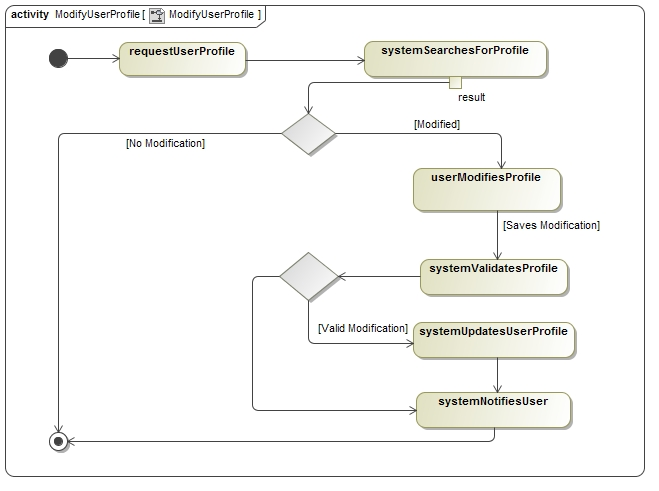
\includegraphics{Images/UserProfile/ModifyUserProfile}
\subsection{Process Specifications:} 
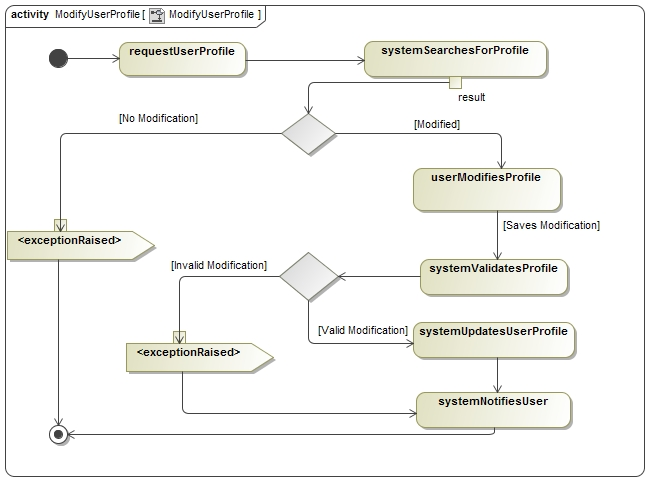
\includegraphics{Images/UserProfile/ModifyUserProfileActivity}

%EPHI
\section{Create Profile}
\subsection*{Description:}
\subsection{Prioritization:} 
\subsection{Conditions and Data Structures:}
\subsubsection*{Pre-Conditions:}
\subsubsection*{Post-Conditions:}
\subsubsection*{Requests and Results Data Structures:}
\subsection{Required Functionality:} 
\subsection{Process Specifications:} 

%.........
\section{Create Private Message}
\subsection*{Description:}
\subsection{Prioritization:} 
\subsection{Conditions and Data Structures:}
\subsubsection*{Pre-Conditions:}
\subsubsection*{Post-Conditions:}
\subsubsection*{Requests and Results Data Structures:}
\subsection{Required Functionality:} 
\subsection{Process Specifications:} 

%.........
\section{Read Private Message}
\subsection*{Description:}
\subsection{Prioritization:} 
\subsection{Conditions and Data Structures:}
\subsubsection*{Pre-Conditions:}
\subsubsection*{Post-Conditions:}
\subsubsection*{Requests and Results Data Structures:}
\subsection{Required Functionality:} 
\subsection{Process Specifications:} 

%.........
\section{Update Private Message}
\subsection*{Description:}
\subsection{Prioritization:} 
\subsection{Conditions and Data Structures:}
\subsubsection*{Pre-Conditions:}
\subsubsection*{Post-Conditions:}
\subsubsection*{Requests and Results Data Structures:}
\subsection{Required Functionality:} 
\subsection{Process Specifications:} 

%.........
\section{Delete Private Message}
\subsection*{Description:}
\subsection{Prioritization:} 
\subsection{Conditions and Data Structures:}
\subsubsection*{Pre-Conditions:}
\subsubsection*{Post-Conditions:}
\subsubsection*{Requests and Results Data Structures:}
\subsection{Required Functionality:} 
\subsection{Process Specifications:} 

%LEAVE
\newpage
\begin{center}
\section*\textbf\huge{Domain Model}
\addcontentsline{toc}{section}{Domain Model}

\end{center}
\setcounter{section}{0}
%---------------------------------------------------------------START EDITING HERE FOR DOMAIN MODEL----------------------------------------------------------------------

\end{document}

